\documentclass[]{beamer}
%for printing or having a crappy pdf reader backup
%\documentclass[handout]{beamer}
\mode<presentation>
\usetheme{Madrid}


\usecolortheme[RGB={80,0,0}]{structure}
%teal \usecolortheme[RGB={0,128,128}]{structure}
\useoutertheme{miniframes}
\useinnertheme{default}
\usepackage{color}
\definecolor{Maroon}{RGB}{80,0,0}
\definecolor{BurntOrange}{RGB}{204,85,0}
\usepackage{setspace}
\usepackage{amsmath}
\usepackage{amsthm}
\usepackage{amsfonts}
\usepackage{amssymb}
\usepackage{verbatim}
\usepackage{array}
\usepackage{graphicx}
\usepackage{subfigure}
\usepackage{colortbl}
%\usepackage[retainorgcmds]{IEEEtrantools}
\usepackage{wrapfig}
\usepackage[figurename=,tablename=]{caption}
\usepackage{multirow}
\setbeamercolor{normal text}{fg=black}
\setbeamercovered{dynamic}
\beamertemplatetransparentcovereddynamicmedium
%\usepackage{chronology}
\setbeamertemplate{caption}[numbered]
\usepackage{colortbl}
\newcommand {\mathsym}[1]{{}}
\newcommand {\unicode}{{}}
\newcommand{\om}{\boldsymbol{\Omega}}
\newcommand{\etal}{{\it et al.\,}}
\newcommand{\vr}{\vec{r}}
\newcommand{\vo}{\vec{\Omega}}
\newcolumntype{L}{>{\centering\arraybackslash}m{3cm}}
\newcommand{\tcr}[1]{\textcolor{red}{#1}}
%Creating a norm command
\newcommand{\norm}[1]{\left\lVert#1\right\rVert}
%Allow page breaks within align
\allowdisplaybreaks
%Code
\usepackage{listings}
\usepackage{pdfpages}
\newlength \figwidth
\setlength \figwidth {0.5\textwidth}

\usepackage[percent]{overpic}



\begin{document}
%

\title[XFEM Moving Interface Verification]{Extended Finite Element Method Development \& Application for Simulation of Moving Interface \& Boundary Phenomena}
\author[Tompkins]{James B. Tompkins \\ Chair: Dr. Ryan G. McClarren \\ Co-chair: Dr. Jean C. Ragusa \\ Committee: Drs. J.N. Reddy \& Lin Shao}
\institute[TAMU]{Texas A\&M University}
%\committee[McClarren,Arroyave,Ragusa,Shao,Hales]{Dr. Ryan McClarren \\ Dr. Raymundo Arr\'{o}yave \\ Dr. Jean Ragusa \\ Dr. Lin Shao \\ Dr. Jason Hales}
\date[Sept 19, 2018]

% ###############################################################################
\section{1D XY Homog}
\subsection{}
% ###############################################################################
\begin{frame}[t]\frametitle{1D, Cartesian, Homogeneous 1 Material Problem Description}
  \begin{block}{PDE}
    $\rho c_p\frac{\partial T}{\partial t} - \nabla k \nabla T = \rho c_p\frac{\partial T}{\partial t} - \frac{\partial}{\partial x} k \frac{\partial T}{\partial x}= q$
  \end{block}
  
  \begin{block}{Domain/Material Properties}
  	$\Omega_x = [0,1], \,\, \rho c_p = 10, \,\, k=1.5$
  \end{block}
  
  \begin{block}{BCs}
    Left:  \textbf{Neumann} -- $\left. \frac{\partial T}{\partial x}\right|_{x=0} = k \cdot 200t$ \\
    Right: \textbf{Dirichlet} -- $T(1,t) = 400$
  \end{block}
  
  \begin{block}{IC}
    \textbf{Constant} -- $T(x,0) = 400$
  \end{block}
\end{frame}

\begin{frame}[t]\frametitle{Method of Manufactured Solutions for 1D, XY, Homogeneous Material Problem}
\begin{block}{Prescribed Solution}
    $T(x,t) = (-200x+200)t + 400$
  \end{block}
  
  \begin{block}{Derived Source}
  $q = 200\,\rho c_p \left(-x+1\right)$
  \end{block}
  
  \begin{block}{Interface Level Set Function}
    $\phi(x,t) = 1 - (x - 0.04) - 0.2t = 1.04 - x - 0.2t$
  \end{block}
\end{frame}

\begin{frame}\frametitle{Numerical Parameters}
  	\begin{columns}
		\column{0.32\linewidth}
			\begin{center}
			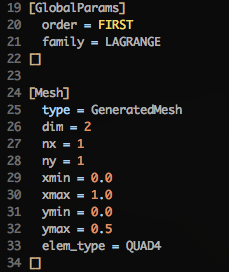
\includegraphics[scale=0.4]{figures/1D_xy_h1m/Screen-GlobalParams-1Dxyh1m}
			\end{center}
		\column{0.66\linewidth}
			\begin{center}
			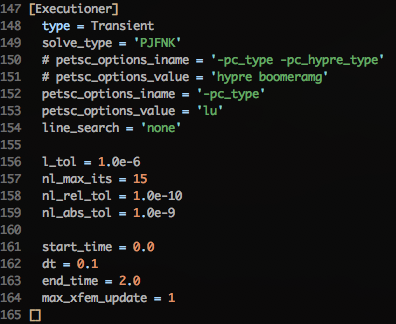
\includegraphics[scale=0.4]{figures/1D_xy_h1m/Screen-Executioner-1Dxyh1m}
			\end{center}
	\end{columns}
	\begin{center}
	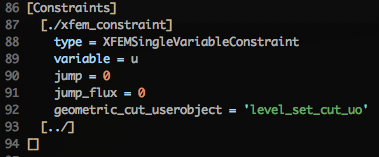
\includegraphics[scale=0.4]{figures/1D_xy_h1m/Screen-Constraints-1Dxyh1m}
	\end{center}
\end{frame}

\begin{frame}[t]\frametitle{Results Comparison}
  	\begin{columns}
		\column{0.48\linewidth}
			\begin{center}
			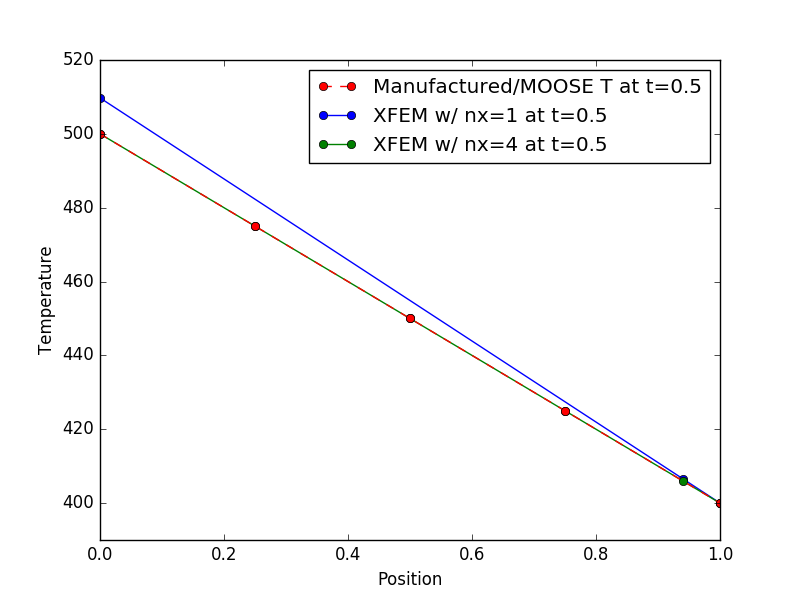
\includegraphics[scale=0.17]{figures/1D_xy_h1m/1D_xy_homog1mat_u_vs_x_05}\\
			$t=0.5$
			
			\null
			
			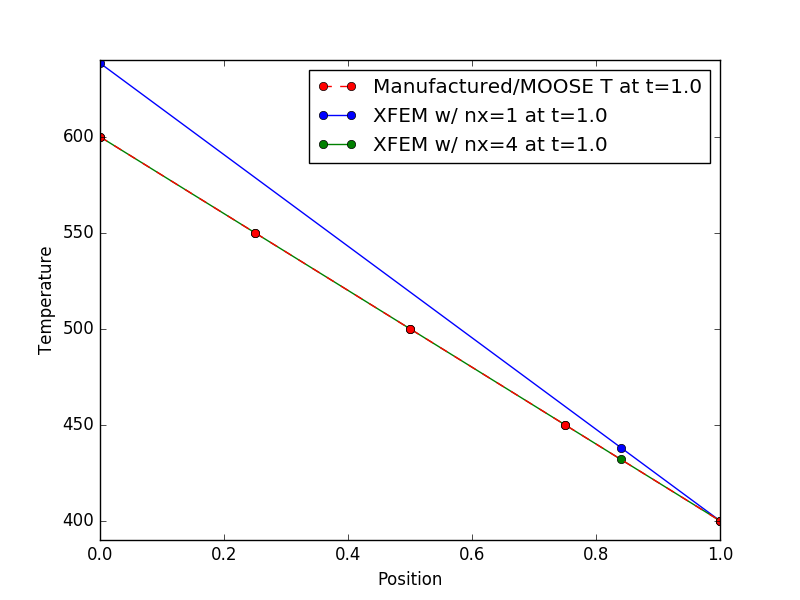
\includegraphics[scale=0.17]{figures/1D_xy_h1m/1D_xy_homog1mat_u_vs_x_10}\\
			$t=1.0$
			\end{center}
		\column{0.48\linewidth}
			\begin{center}
			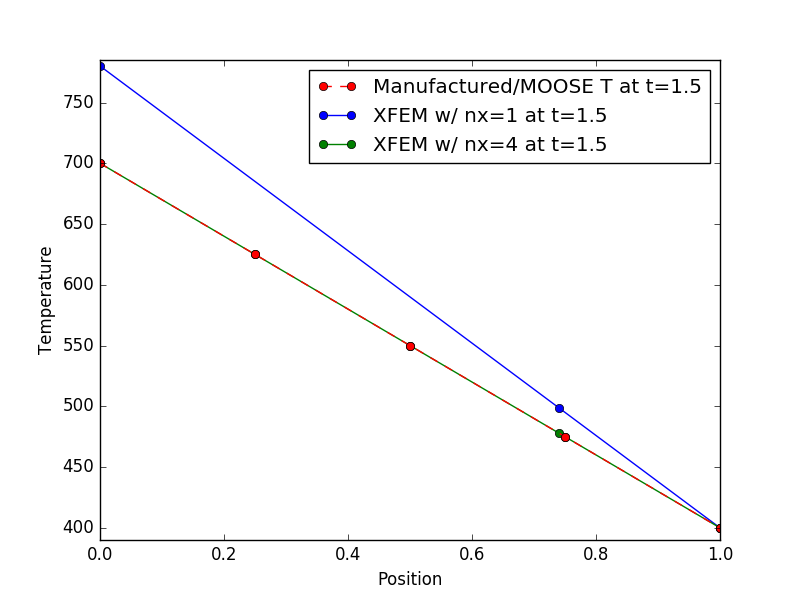
\includegraphics[scale=0.17]{figures/1D_xy_h1m/1D_xy_homog1mat_u_vs_x_15}\\
			$t=1.5$			
			
			\null
			
			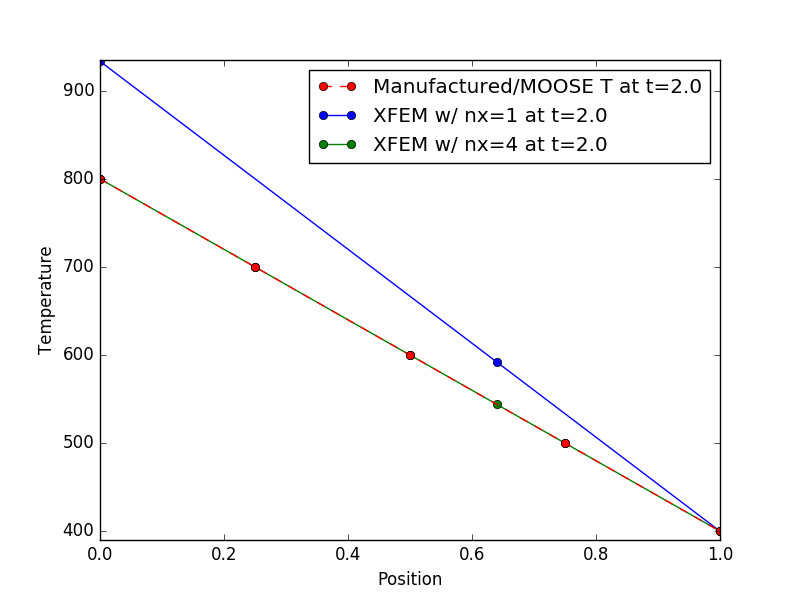
\includegraphics[scale=0.17]{figures/1D_xy_h1m/1D_xy_homog1mat_u_vs_x_20}\\
			$t=2.0$
			\end{center}
	\end{columns}
\end{frame}

\begin{frame}[t]\frametitle{L2 Error Norms at Each Timestep}
  	\begin{columns}
		\column{0.5\linewidth}
			\begin{center}
			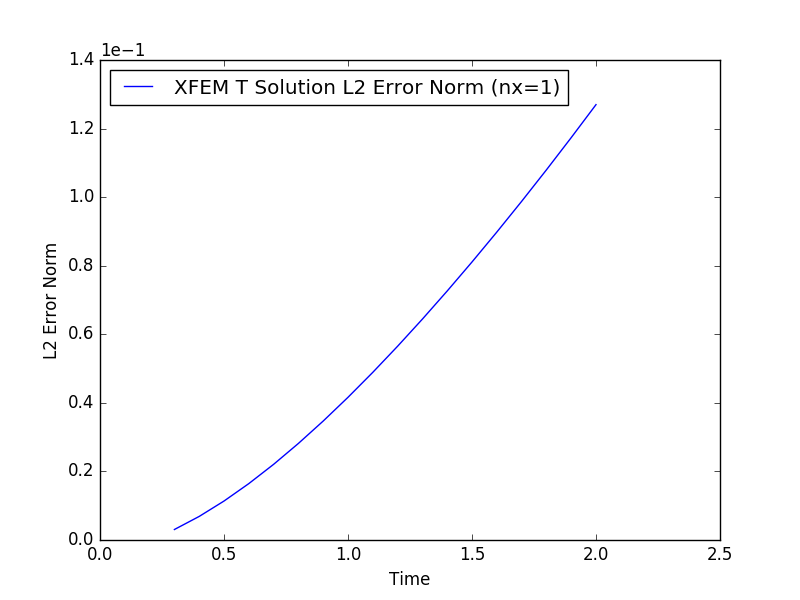
\includegraphics[scale=0.3]{figures/1D_xy_h1m/1D_xy_homog1mat_nx1_L2_Errs}
			\end{center}
		\column{0.5\linewidth}
			\begin{center}
			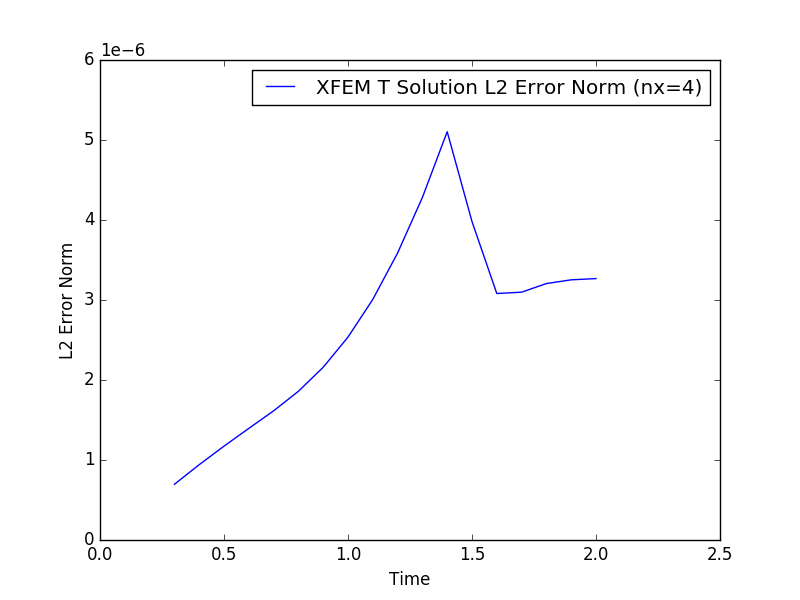
\includegraphics[scale=0.3]{figures/1D_xy_h1m/1D_xy_homog1mat_nx4_L2_Errs}
			\end{center}
	\end{columns}
\end{frame}

\begin{frame}[t]\frametitle{Mesh Refinement Effects on Error at x=0}
	\begin{center}
		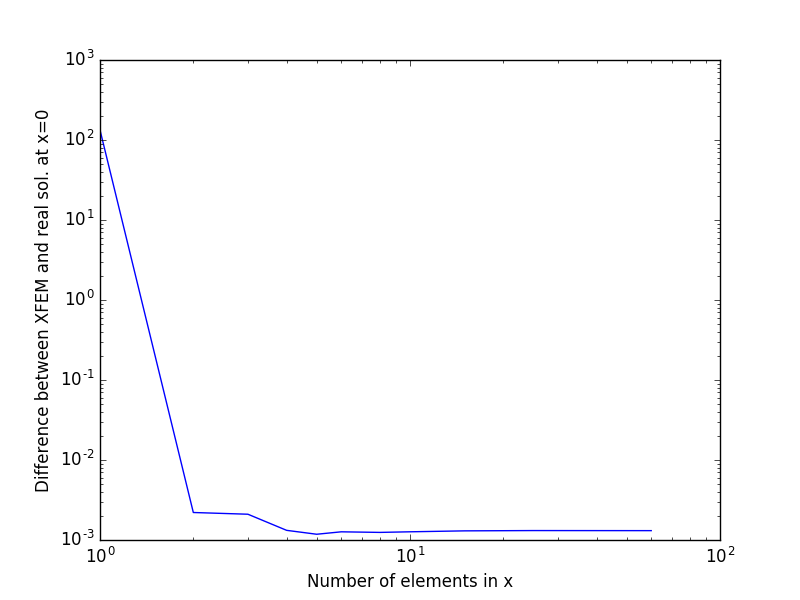
\includegraphics[scale=0.4]{figures/1D_xy_h1m/1D_xy_homog1mat_neumann_comp}
	\end{center}
\end{frame}

% ###############################################################################
\section{1D XY LS Dep}
\subsection{}
% ###############################################################################
\begin{frame}[t]\frametitle{1D, Cartesian, Level Set Dependent Material Problem Description}
  \begin{block}{PDE}
    $\rho c_p\frac{\partial T}{\partial t} - \nabla k \nabla T = \rho c_p\frac{\partial T}{\partial t} - \frac{\partial}{\partial x} k \frac{\partial T}{\partial x}= q$
  \end{block}
  
  \begin{block}{Domain/Material Properties}
  	$\Omega_x = [0,1], \,\, \rho c_p = 10, \,\, k=\left(\frac{0.05}{1.04}\right) \phi(x,t) + 1.5
  	= \frac{0.05}{1.04}\left( - x - 0.2t\right) + 1.55$
  \end{block}
  
  \begin{block}{BCs}
    Left:  \textbf{Neumann} -- $\left. \frac{\partial T}{\partial x}\right|_{x=0} = k(x,t) \cdot 200t$ \\
    Right: \textbf{Dirichlet} -- $T(1,t) = 400$
  \end{block}
  
  \begin{block}{IC}
    \textbf{Constant} -- $T(x,0) = 400$
  \end{block}
\end{frame}

\begin{frame}[t]\frametitle{Method of Manufactured Solutions for 1D, XY, LS Dependent Material Problem}
\begin{block}{Prescribed Solution}
    $T(x,t) = (-200x+200)t + 400$
  \end{block}
  
  \begin{block}{Derived Source}
  $q = 200\,\rho c_p \left(-x+1\right) - \left(\frac{0.05 \cdot 200t}{1.04}\right)$
  \end{block}
  
  \begin{block}{Interface Level Set Function}
    $\phi(x,t) = 1 - (x - 0.04) - 0.2t = 1.04 - x - 0.2t$
  \end{block}
\end{frame}

\begin{frame}\frametitle{Numerical Parameters}
  	\begin{columns}
		\column{0.32\linewidth}
			\begin{center}
			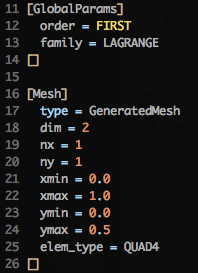
\includegraphics[scale=0.4]{figures/1D_xy_ls1m/Screen-GlobalParams-1Dxyls1m}
			\end{center}
		\column{0.66\linewidth}
			\begin{center}
			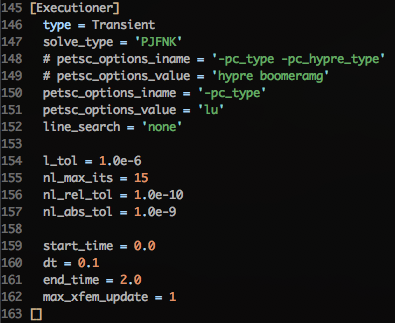
\includegraphics[scale=0.4]{figures/1D_xy_ls1m/Screen-Executioner-1Dxyls1m}
			\end{center}
	\end{columns}
	\begin{center}
	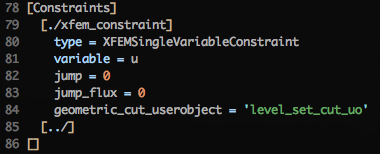
\includegraphics[scale=0.4]{figures/1D_xy_ls1m/Screen-Constraints-1Dxyls1m}
	\end{center}
\end{frame}

\begin{frame}[t]\frametitle{Results Comparison}
  	\begin{columns}
		\column{0.48\linewidth}
			\begin{center}
			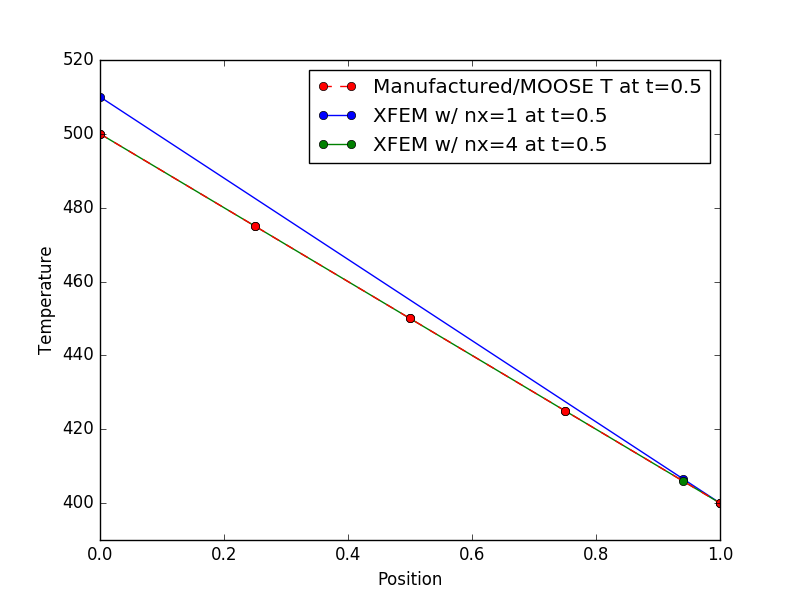
\includegraphics[scale=0.17]{figures/1D_xy_ls1m/1D_xy_ls1mat_u_vs_x_05}\\
			$t=0.5$
			
			\null
			
			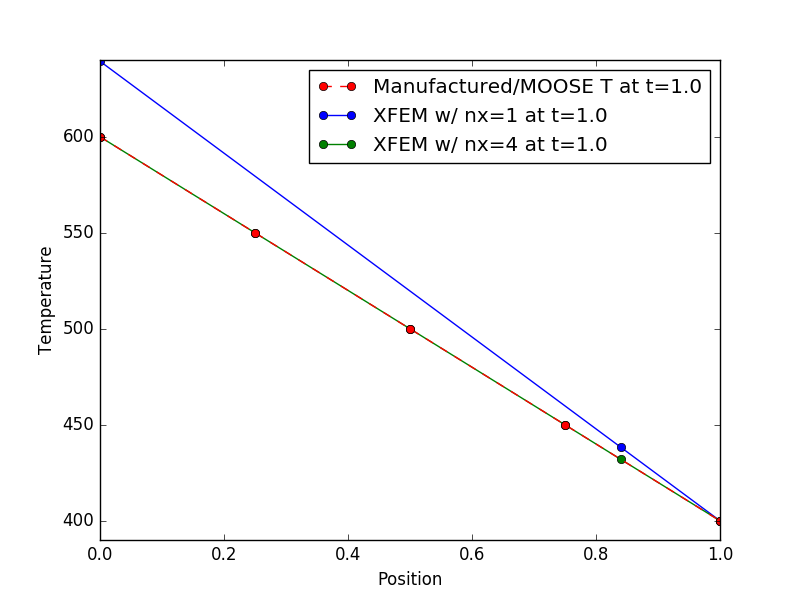
\includegraphics[scale=0.17]{figures/1D_xy_ls1m/1D_xy_ls1mat_u_vs_x_10}\\
			$t=1.0$
			\end{center}
		\column{0.48\linewidth}
			\begin{center}
			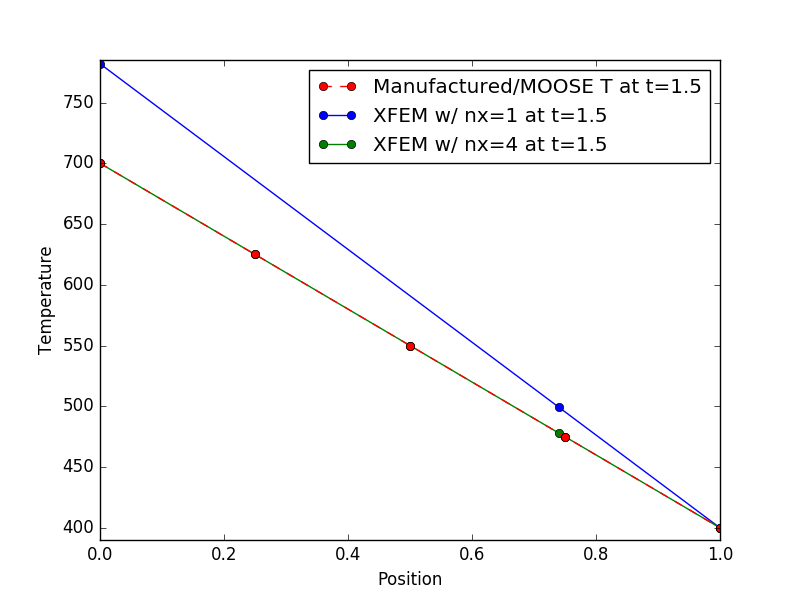
\includegraphics[scale=0.17]{figures/1D_xy_ls1m/1D_xy_ls1mat_u_vs_x_15}\\
			$t=1.5$			
			
			\null
			
			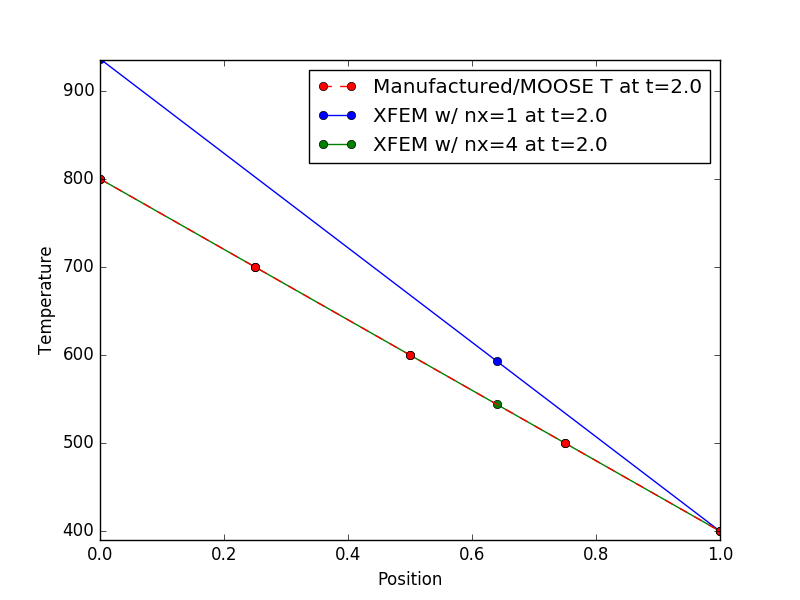
\includegraphics[scale=0.17]{figures/1D_xy_ls1m/1D_xy_ls1mat_u_vs_x_20}\\
			$t=2.0$
			\end{center}
	\end{columns}
\end{frame}

\begin{frame}[t]\frametitle{L2 Error Norms at Each Timestep}
  	\begin{columns}
		\column{0.5\linewidth}
			\begin{center}
			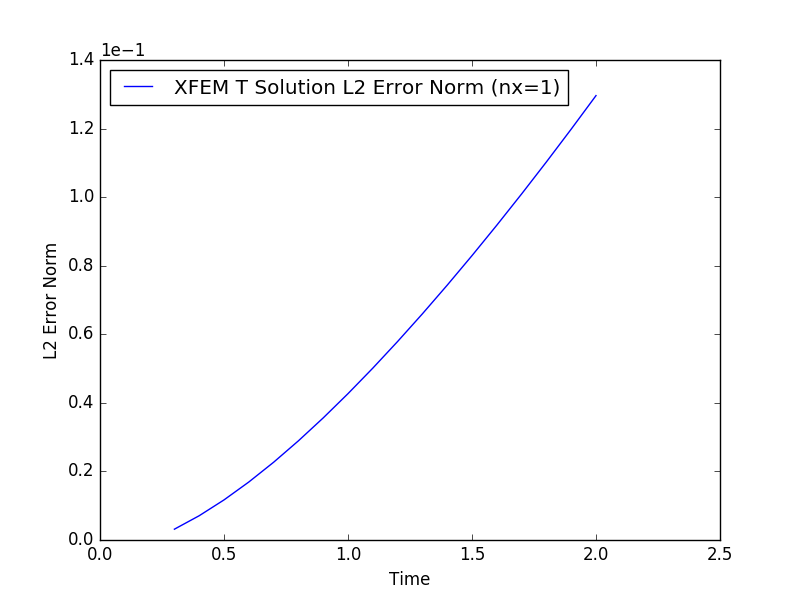
\includegraphics[scale=0.3]{figures/1D_xy_ls1m/1D_xy_ls1mat_nx1_L2_Errs}
			\end{center}
		\column{0.5\linewidth}
			\begin{center}
			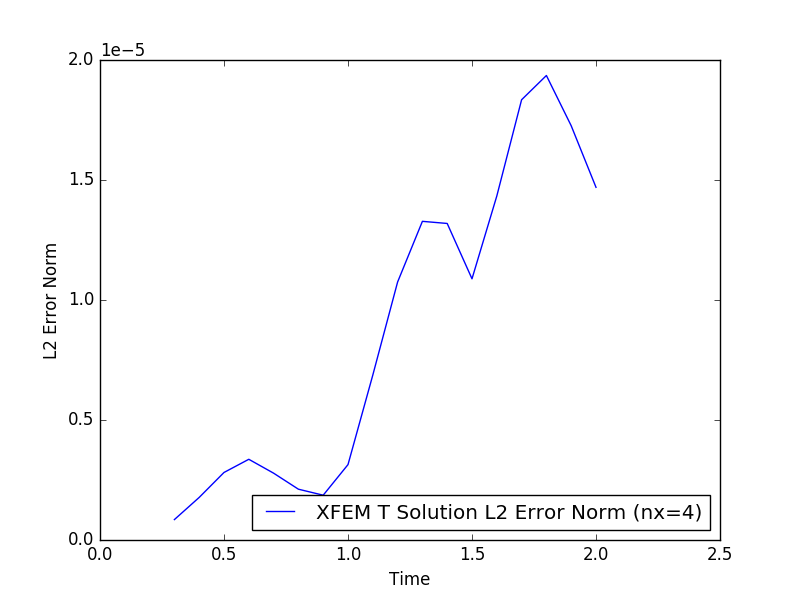
\includegraphics[scale=0.3]{figures/1D_xy_ls1m/1D_xy_ls1mat_nx4_L2_Errs}
			\end{center}
	\end{columns}
\end{frame}

\begin{frame}[t]\frametitle{Mesh Refinement Effects on Error at x=0}
	\begin{center}
		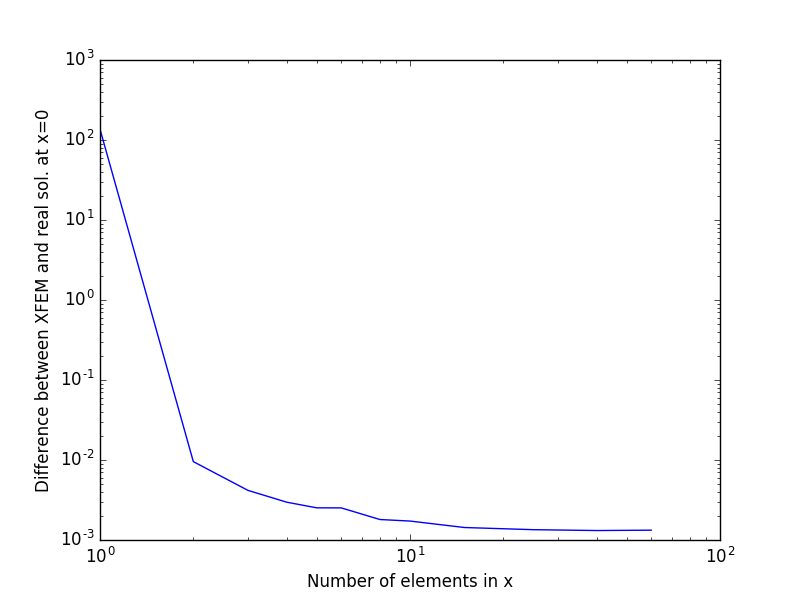
\includegraphics[scale=0.4]{figures/1D_xy_ls1m/1D_xy_ls1mat_neumann_comp}
	\end{center}
\end{frame}

% ###############################################################################
\section{1D RZ Homog}
\subsection{}
% ###############################################################################
\begin{frame}[t]\frametitle{1D, Cylindrical, Homogeneous Material Problem Description}
  \begin{block}{PDE}
    $\rho c_p\frac{\partial T}{\partial t} - \nabla k \nabla T = \rho c_p\frac{\partial T}{\partial t} - \frac{1}{r} \frac{\partial}{\partial r}\left(r\cdot k \frac{\partial T}{\partial r} \right) = q$
  \end{block}
  
  \begin{block}{Domain/Material Properties}
  	$\Omega_r = [1,2], \,\,\ \rho c_p = 10, \,\, k = 1.5$
  \end{block}
  
  \begin{block}{BCs}
    Left:  \textbf{Neumann} -- $\left. \frac{\partial T}{\partial r}\right|_{r=1} = k \cdot 200t$ \\
    Right: \textbf{Dirichlet} -- $T(2,t) = 400$
  \end{block}
  
  \begin{block}{ICs}
    \textbf{Constant} -- $T(r,0) = 400$
  \end{block}
\end{frame}

\begin{frame}[t]\frametitle{Method of Manufactured Solutions for 1D, RZ, Homogeneous Material Problem}
  \begin{block}{Prescribed Solution}
    $T(r,t) = (-200r+400)t + 400$
  \end{block}
  
  \begin{block}{Derived Source}
  $q = 200\,\rho c_p \left(-x+2\right) + \frac{200kt}{r}$
  \end{block}
  
  \begin{block}{Interface Level Set Function}
    $\phi(r,t) = 2 - (r - 0.04) - 0.2t = 2.04 - r - 0.2t$
  \end{block}
\end{frame}

\begin{frame}\frametitle{Numerical Parameters}
  	\begin{columns}
		\column{0.32\linewidth}
			\begin{center}
			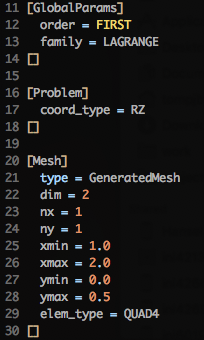
\includegraphics[scale=0.4]{figures/1D_rz_h1m/Screen-GlobalParams-1Drzh1m}
			\end{center}
		\column{0.66\linewidth}
			\begin{center}
			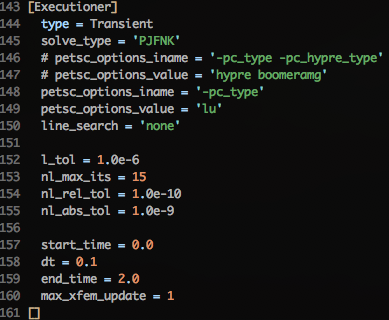
\includegraphics[scale=0.4]{figures/1D_rz_h1m/Screen-Executioner-1Drzh1m}
			\end{center}
	\end{columns}
	\begin{center}
	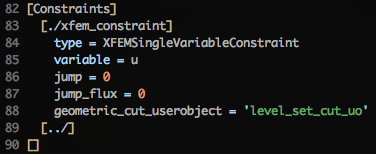
\includegraphics[scale=0.4]{figures/1D_rz_h1m/Screen-Constraints-1Drzh1m}
	\end{center}
\end{frame}

\begin{frame}[t]\frametitle{Results Comparison}
  	\begin{columns}
		\column{0.48\linewidth}
			\begin{center}
			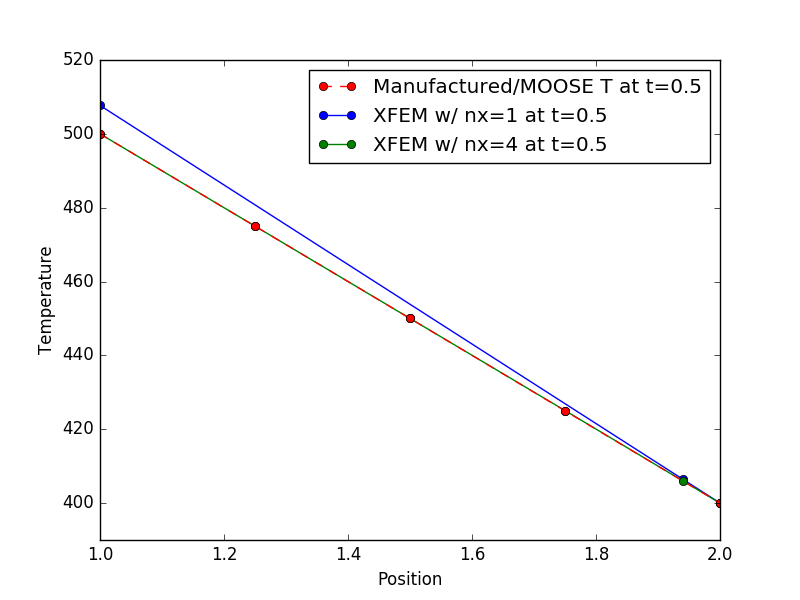
\includegraphics[scale=0.17]{figures/1D_rz_h1m/1D_rz_homog1mat_u_vs_x_05}\\
			$t=0.5$
			
			\null
			
			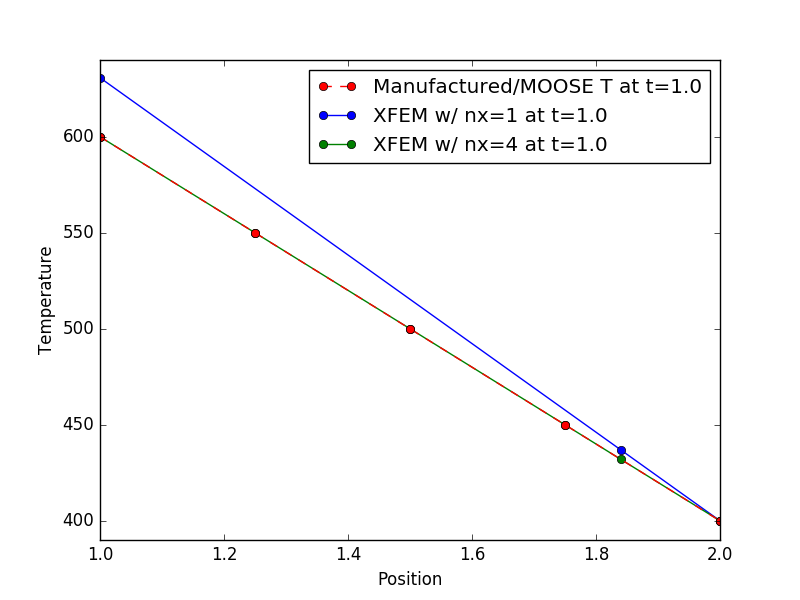
\includegraphics[scale=0.17]{figures/1D_rz_h1m/1D_rz_homog1mat_u_vs_x_10}\\
			$t=1.0$
			\end{center}
		\column{0.48\linewidth}
			\begin{center}
			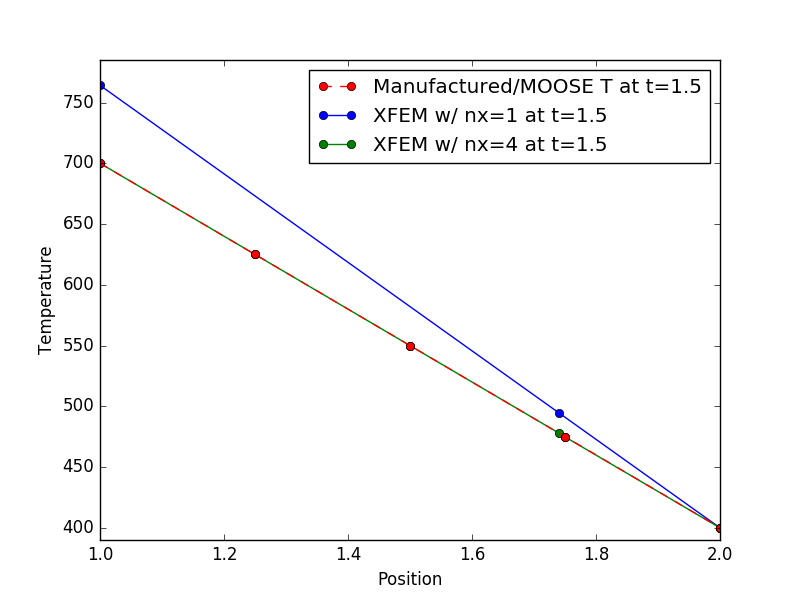
\includegraphics[scale=0.17]{figures/1D_rz_h1m/1D_rz_homog1mat_u_vs_x_15}\\
			$t=1.5$			
			
			\null
			
			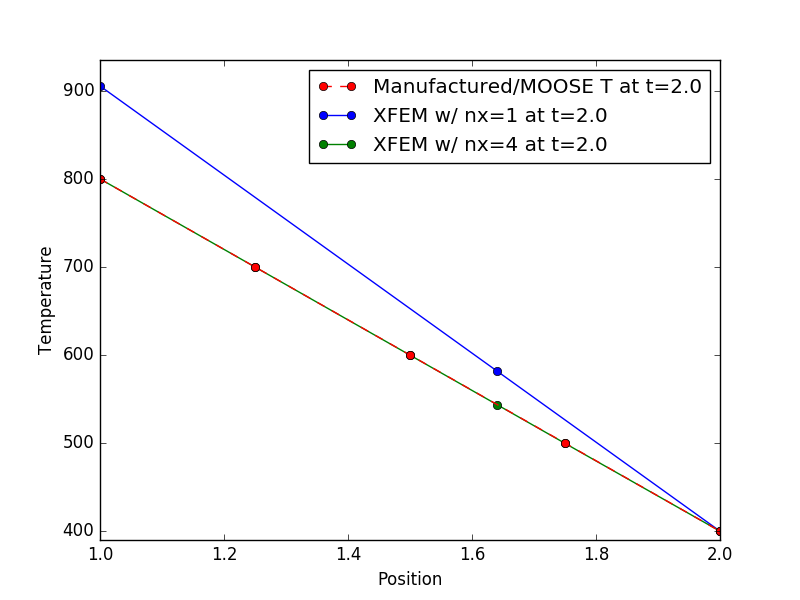
\includegraphics[scale=0.17]{figures/1D_rz_h1m/1D_rz_homog1mat_u_vs_x_20}\\
			$t=2.0$
			\end{center}
	\end{columns}
\end{frame}

\begin{frame}[t]\frametitle{L2 Error Norms at Each Timestep}
  	\begin{columns}
		\column{0.5\linewidth}
			\begin{center}
			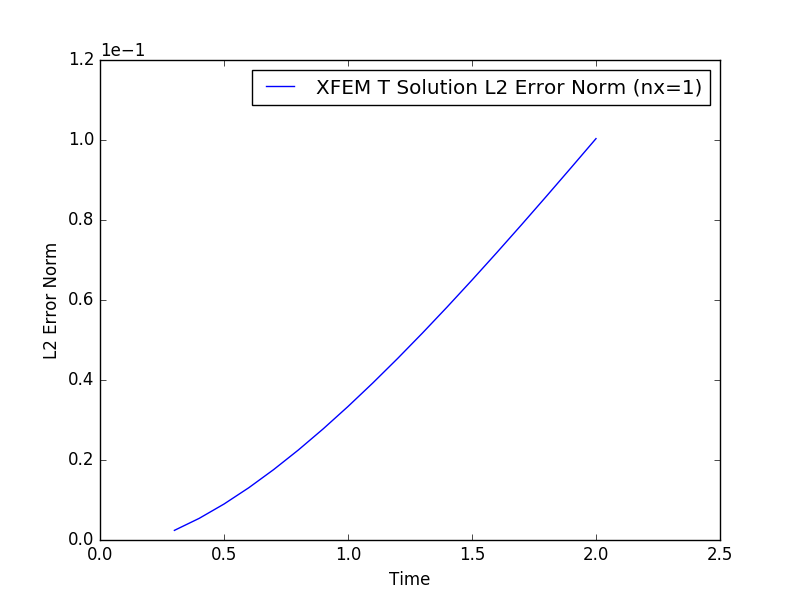
\includegraphics[scale=0.3]{figures/1D_rz_h1m/1D_rz_homog1mat_nx1_L2_Errs}
			\end{center}
		\column{0.5\linewidth}
			\begin{center}
			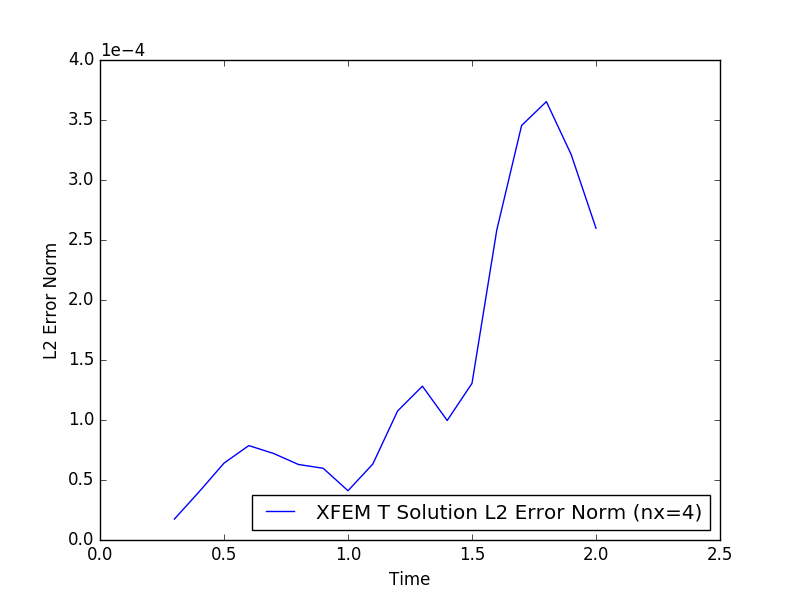
\includegraphics[scale=0.3]{figures/1D_rz_h1m/1D_rz_homog1mat_nx4_L2_Errs}
			\end{center}
	\end{columns}
\end{frame}

\begin{frame}[t]\frametitle{Mesh Refinement Effects on Error at x=1}
	\begin{center}
		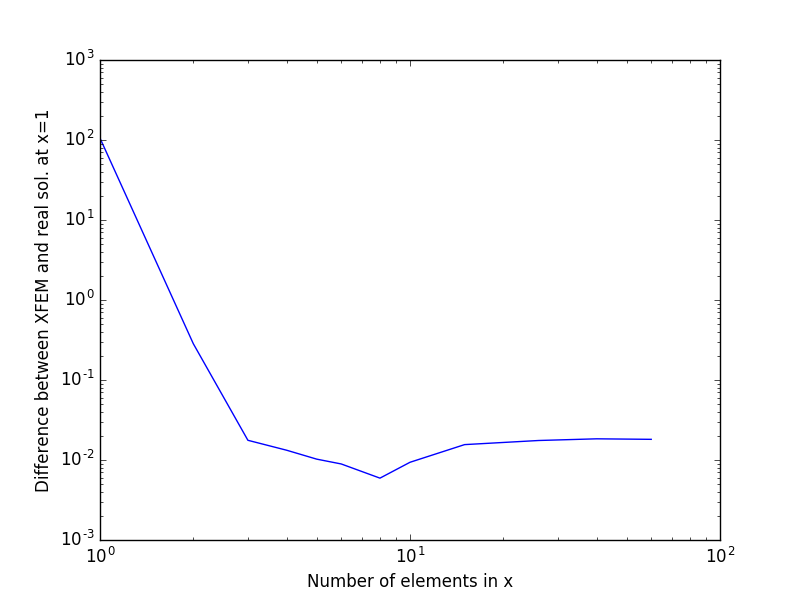
\includegraphics[scale=0.4]{figures/1D_rz_h1m/1D_rz_homog1mat_neumann_comp}
	\end{center}
\end{frame}

% ###############################################################################
\section{1D RZ LS Dep}
\subsection{}
% ###############################################################################
\begin{frame}[t]\frametitle{1D, Cylindrical, Level Set Dependent Material Problem Description}
  \begin{block}{PDE}
    $\rho c_p\frac{\partial T}{\partial t} - \nabla k \nabla T = \rho c_p\frac{\partial T}{\partial t} - \frac{1}{r} \frac{\partial}{\partial r}\left(r\cdot k \frac{\partial T}{\partial r} \right) = q$
  \end{block}
  
  \begin{block}{Domain/Material Properties}
  	$\Omega_r = [1,2], \,\,\ \rho c_p = 10, \,\, k=\left(\frac{0.05}{2.04}\right) \phi(x,t) + 1.5
  	= \frac{0.05}{2.04}\left( - x - 0.2t\right) + 1.55$
  \end{block}
  
  \begin{block}{BCs}
    Left:  \textbf{Neumann} -- $\left. \frac{\partial T}{\partial r}\right|_{r=1} = k(r,t) \cdot 200t$ \\
    Right: \textbf{Dirichlet} -- $T(2,t) = 400$
  \end{block}
  
  \begin{block}{ICs}
    \textbf{Constant} -- $T(r,0) = 400$
  \end{block}
\end{frame}

\begin{frame}[t]\frametitle{Method of Manufactured Solutions for 1D, RZ, LS Dependent Material Problem}
  \begin{block}{Prescribed Solution}
    $T(r,t) = (-200r+400)t + 400$
  \end{block}
  
  \begin{block}{Derived Source}
  $q = 200\,\rho c_p \left(-x+2\right) + \frac{1}{r}\left( 310t - \frac{10rt}{1.02} - \frac{t^2}{1.02}\right)$
  \end{block}
  
  \begin{block}{Interface Level Set Function}
    $\phi(r,t) = 2 - (r - 0.04) - 0.2t = 2.04 - r - 0.2t$
  \end{block}
\end{frame}

\begin{frame}\frametitle{Numerical Parameters}
  	\begin{columns}
		\column{0.32\linewidth}
			\begin{center}
			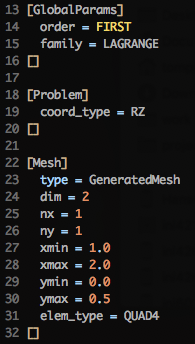
\includegraphics[scale=0.4]{figures/1D_rz_ls1m/Screen-GlobalParams-1Drzls1m}
			\end{center}
		\column{0.66\linewidth}
			\begin{center}
			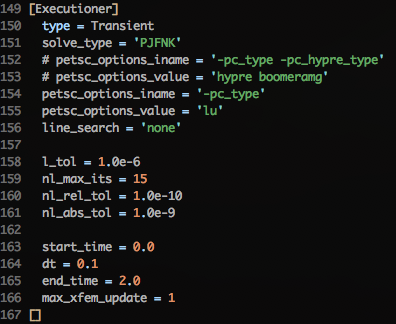
\includegraphics[scale=0.4]{figures/1D_rz_ls1m/Screen-Executioner-1Drzls1m}
			\end{center}
	\end{columns}
	\begin{center}
	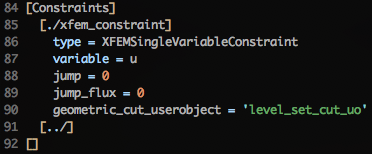
\includegraphics[scale=0.4]{figures/1D_rz_ls1m/Screen-Constraints-1Drzls1m}
	\end{center}
\end{frame}

\begin{frame}[t]\frametitle{Results Comparison}
  	\begin{columns}
		\column{0.48\linewidth}
			\begin{center}
			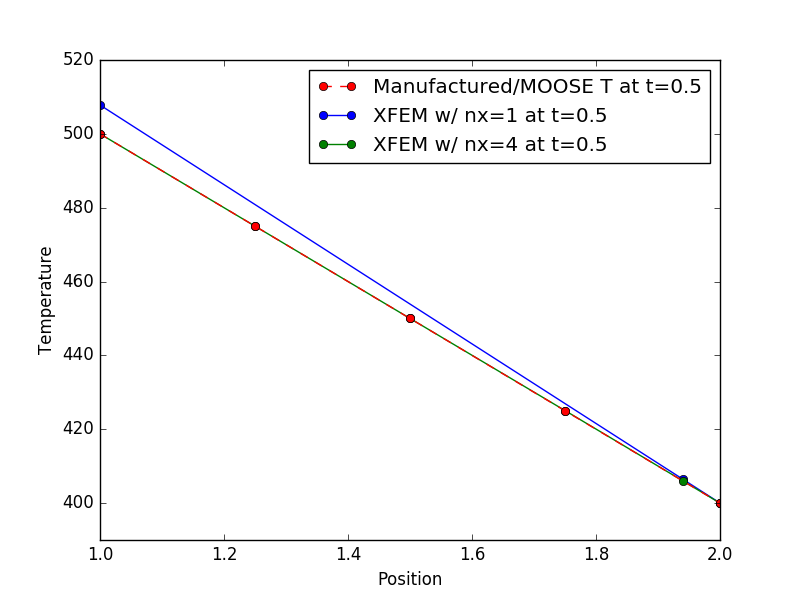
\includegraphics[scale=0.17]{figures/1D_rz_ls1m/1D_rz_ls1mat_u_vs_x_05}\\
			$t=0.5$
			
			\null
			
			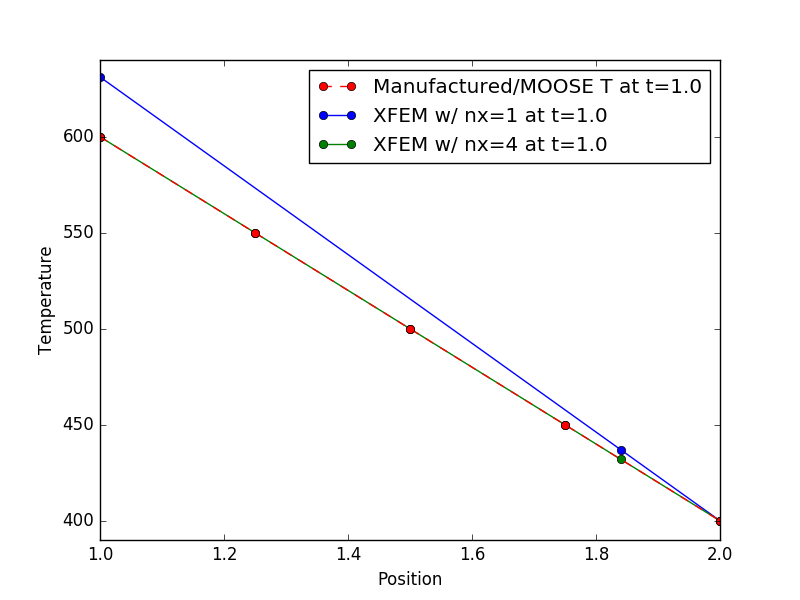
\includegraphics[scale=0.17]{figures/1D_rz_ls1m/1D_rz_ls1mat_u_vs_x_10}\\
			$t=1.0$
			\end{center}
		\column{0.48\linewidth}
			\begin{center}
			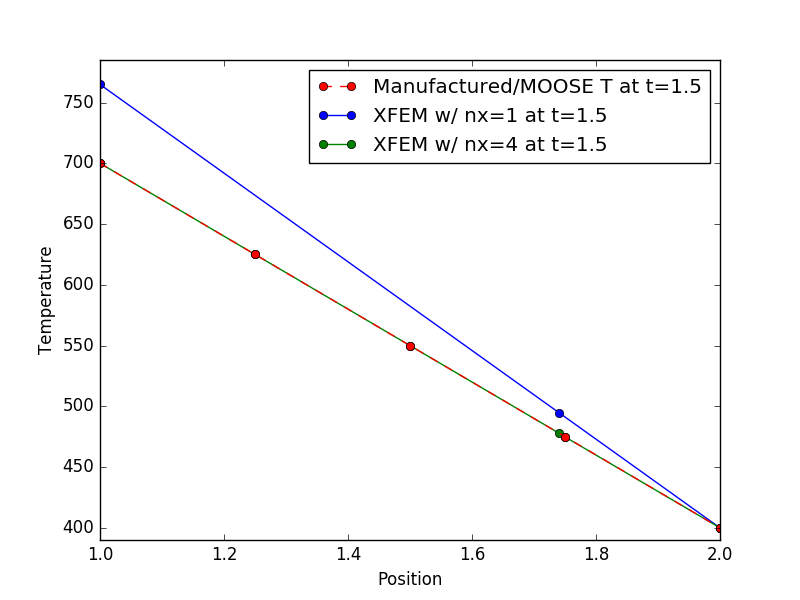
\includegraphics[scale=0.17]{figures/1D_rz_ls1m/1D_rz_ls1mat_u_vs_x_15}\\
			$t=1.5$			
			
			\null
			
			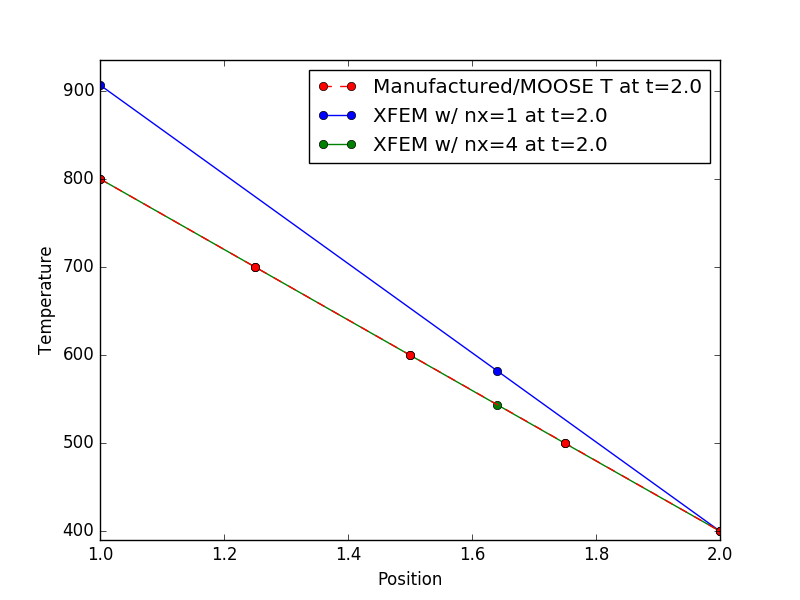
\includegraphics[scale=0.17]{figures/1D_rz_ls1m/1D_rz_ls1mat_u_vs_x_20}\\
			$t=2.0$
			\end{center}
	\end{columns}
\end{frame}

\begin{frame}[t]\frametitle{L2 Error Norms at Each Timestep}
  	\begin{columns}
		\column{0.5\linewidth}
			\begin{center}
			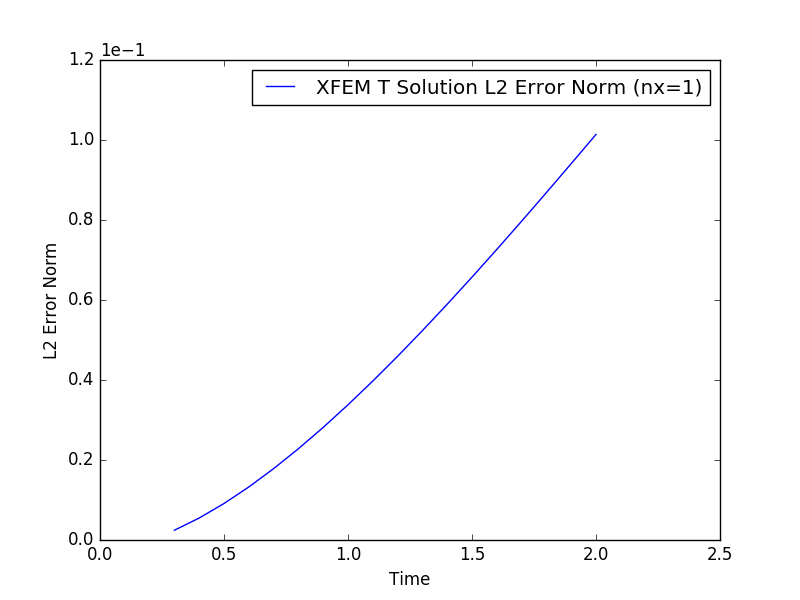
\includegraphics[scale=0.3]{figures/1D_rz_ls1m/1D_rz_ls1mat_nx1_L2_Errs}
			\end{center}
		\column{0.5\linewidth}
			\begin{center}
			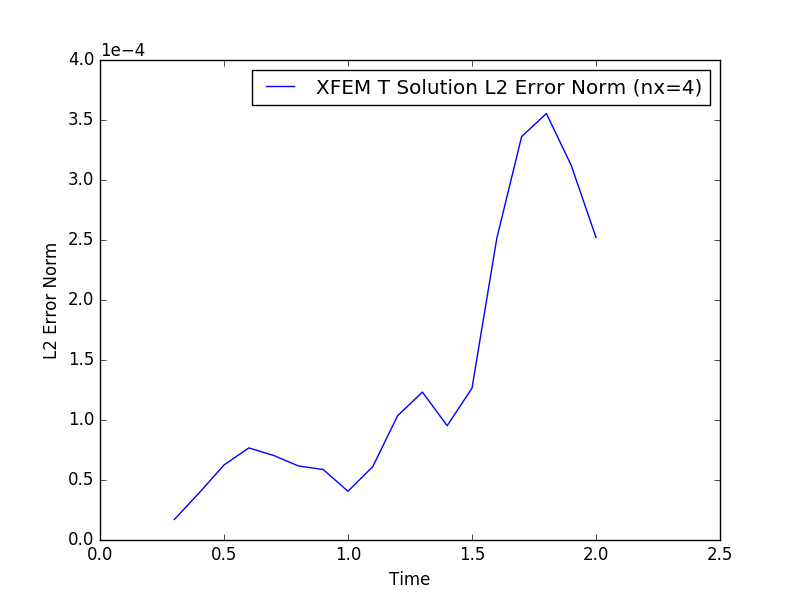
\includegraphics[scale=0.3]{figures/1D_rz_ls1m/1D_rz_ls1mat_nx4_L2_Errs}
			\end{center}
	\end{columns}
\end{frame}

\begin{frame}[t]\frametitle{Mesh Refinement Effects on Error at x=1}
	\begin{center}
		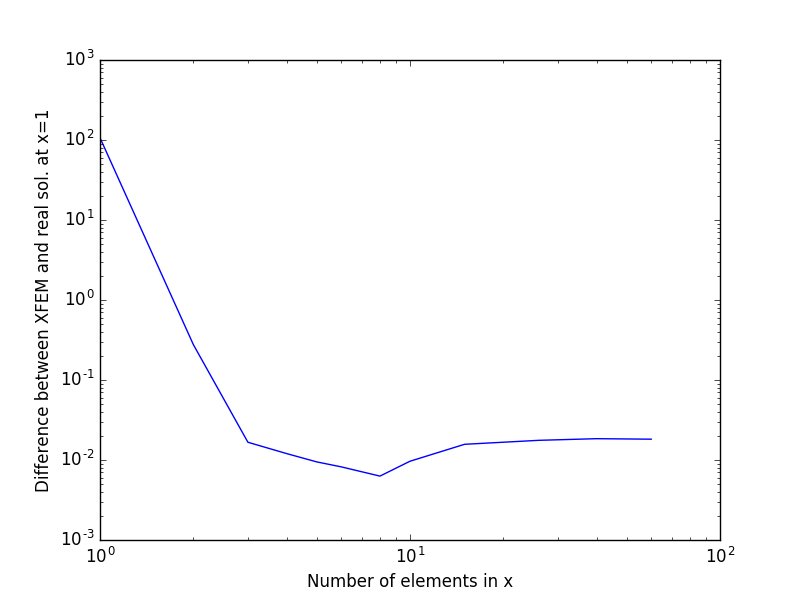
\includegraphics[scale=0.4]{figures/1D_rz_ls1m/1D_rz_ls1mat_neumann_comp}
	\end{center}
\end{frame}

% ###############################################################################
\section{2D XY Homog}
\subsection{}
% ###############################################################################
\begin{frame}[t]\frametitle{2D, Cartesian, Homogeneous Material Problem Description}
  \begin{block}{PDE}
    $\rho c_p\frac{\partial T}{\partial t} - \nabla k \nabla T = 
    \rho c_p\frac{\partial T}{\partial t} - \frac{\partial}{\partial x}
    \left(k\frac{\partial T}{\partial x}\right) - \frac{\partial}{\partial y}
    \left(k\frac{\partial T}{\partial y}\right)= q$
  \end{block}
  
  \begin{block}{Domain/Material Properties}
  	$[\Omega_x,\Omega_y] = [[0,1],[0,1]]$ \\
  	$\rho c_p = 10$ \\
  	$k=1.5$
  \end{block}
\end{frame}
  
\begin{frame}[t]\frametitle{2D, Cartesian, Homogeneous Material Problem BCs/IC}
  \begin{block}{BCs}
    Left: \textbf{Neumann} -- $\left. \frac{\partial T}{\partial x}\right|_{x=0} = k\cdot 100t$ \\
    Right: \textbf{Dirichlet} -- $T(1,y,t) = (-100y + 100)t +400$ \\
    Bottom: \textbf{Neumann} -- $\left. \frac{\partial T}{\partial y}\right|_{y=0} = k\cdot 100t$ \\
    Top: \textbf{Dirichlet} -- $T(x,1,t) = (-100x + 100)t + 400 $
  \end{block}
  
  \begin{block}{ICs}
    \textbf{Constant} -- $T(x,y,0) = 400$
  \end{block}
\end{frame}

\begin{frame}[t]\frametitle{Method of Manufactured Solutions for 2D, XY, Homogeneous Material Problem}
  \begin{block}{Prescribed Solution}
    $T(x,t) = (-100x-100y+200)t + 400$
  \end{block}
  
  \begin{block}{Derived Source}
  $q = 100\,\rho c_p \left(-x-y+2\right)$
  \end{block}
  
  \begin{block}{Interface Level Set Function}
    $\phi(x,y,t) = -0.5(x+y) + 1.04 - 0.2t$
  \end{block}
\end{frame}

\begin{frame}\frametitle{Numerical Parameters}
  	\begin{columns}
		\column{0.32\linewidth}
			\begin{center}
			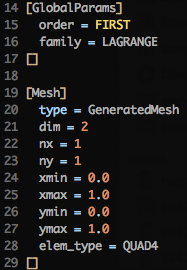
\includegraphics[scale=0.4]{figures/2D_xy_h1m/Screen-GlobalParams-2Dxyh1m}
			\end{center}
		\column{0.66\linewidth}
			\begin{center}
			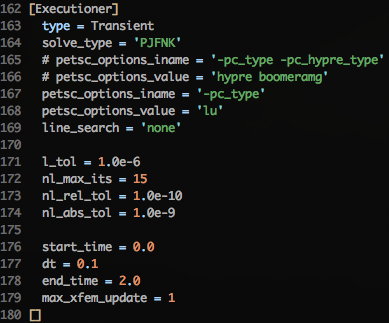
\includegraphics[scale=0.4]{figures/2D_xy_h1m/Screen-Executioner-2Dxyh1m}
			\end{center}
	\end{columns}
	\begin{center}
	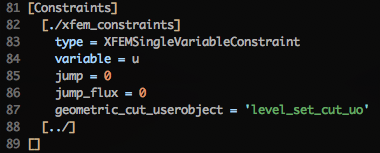
\includegraphics[scale=0.4]{figures/2D_xy_h1m/Screen-Constraints-2Dxyh1m}
	\end{center}
\end{frame}

\begin{frame}[t]\frametitle{Results Comparison}
  Upper plane is nx=1, ny=1; lower plane is nx=4, ny=4
  	\begin{columns}
		\column{0.48\linewidth}
			\begin{center}
			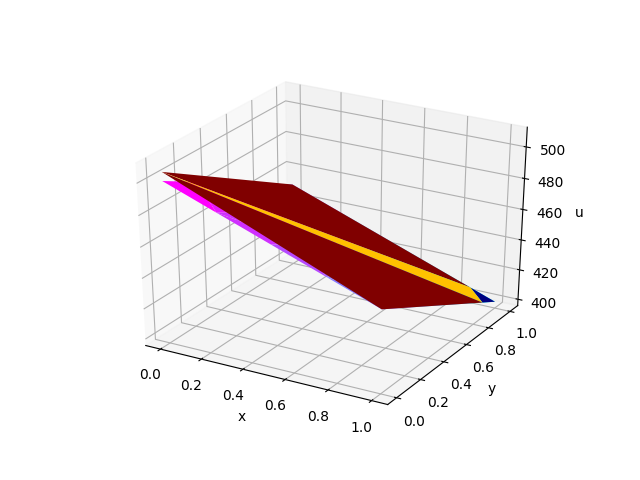
\includegraphics[scale=0.2]{figures/2D_xy_h1m/2D_xy_homog1mat_u_vs_x_05}\\
			\tiny$t=0.5$
			
			\null
			
			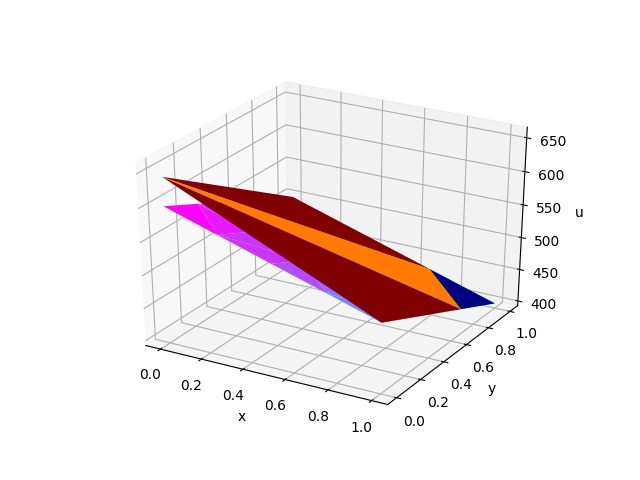
\includegraphics[scale=0.2]{figures/2D_xy_h1m/2D_xy_homog1mat_u_vs_x_10}\\
			$t=1.0$
			\end{center}
		\column{0.48\linewidth}
			\begin{center}
			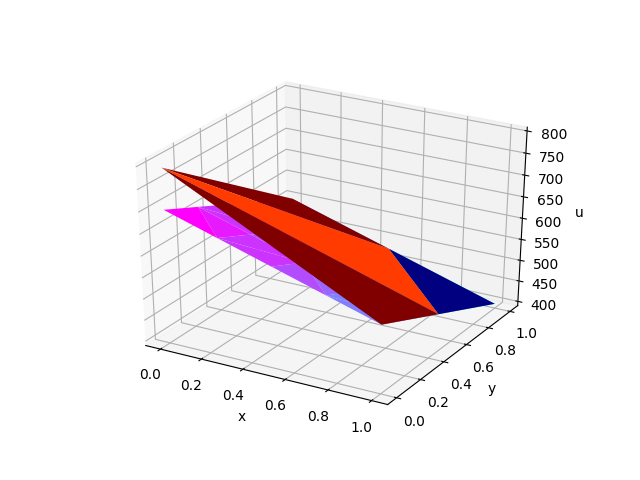
\includegraphics[scale=0.2]{figures/2D_xy_h1m/2D_xy_homog1mat_u_vs_x_15}\\
			\tiny$t=1.5$			
			
			\null
			
			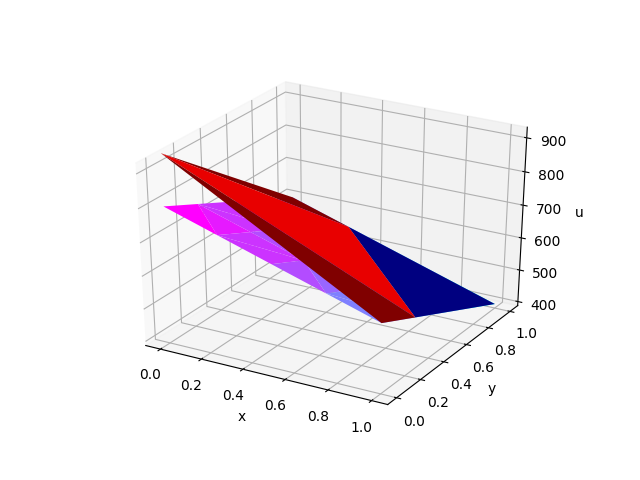
\includegraphics[scale=0.2]{figures/2D_xy_h1m/2D_xy_homog1mat_u_vs_x_20}\\
			$t=2.0$ \normalsize
			\end{center}
	\end{columns}
\end{frame}

\begin{frame}[t]\frametitle{L2 Error Norms at Each Timestep}
  	\begin{columns}
		\column{0.5\linewidth}
			\begin{center}
			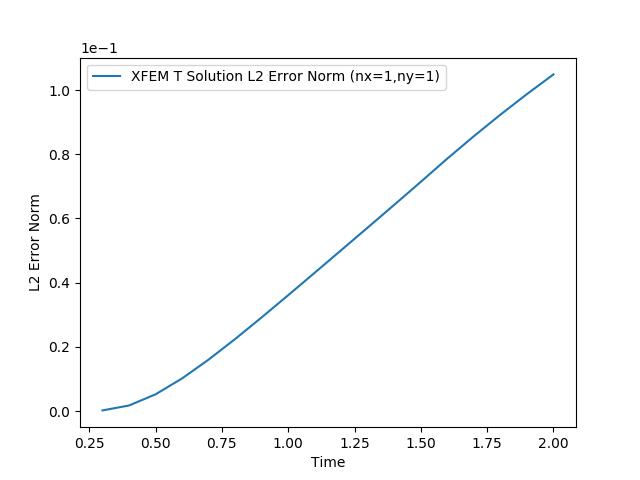
\includegraphics[scale=0.4]{figures/2D_xy_h1m/2D_xy_homog1mat_nx1ny1_L2_Errs}
			\end{center}
		\column{0.5\linewidth}
			\begin{center}
			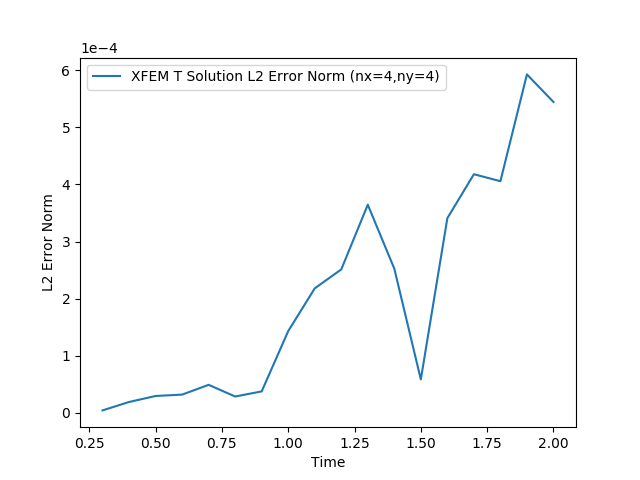
\includegraphics[scale=0.4]{figures/2D_xy_h1m/2D_xy_homog1mat_nx4ny4_L2_Errs}
			\end{center}
	\end{columns}
\end{frame}

\begin{frame}[t]\frametitle{Mesh Refinement Effects on Error at x=0,y=0}
	\begin{center}
		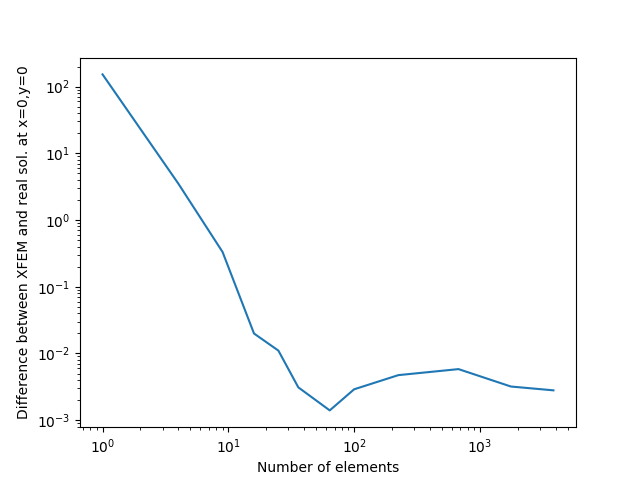
\includegraphics[scale=0.5]{figures/2D_xy_h1m/2D_xy_homog1mat_neumann_comp}
	\end{center}
\end{frame}

% ###############################################################################
\section{2D XY LS Dep}
\subsection{}
% ###############################################################################
\begin{frame}[t]\frametitle{2D, Cartesian, Level Set Dependent Material Problem Description}
  \begin{block}{PDE}
    $\rho c_p\frac{\partial T}{\partial t} - \nabla k \nabla T = 
    \rho c_p\frac{\partial T}{\partial t} - \frac{\partial}{\partial x}
    \left(k\frac{\partial T}{\partial x}\right) - \frac{\partial}{\partial y}
    \left(k\frac{\partial T}{\partial y}\right)= q$
  \end{block}
  
  \begin{block}{Domain/Material Properties}
  	$[\Omega_x,\Omega_y] = [[0,1],[0,1]]$ \\
  	$\rho c_p = 10$ \\
  	$k(x,y,t) = \left(\frac{0.05}{1.04} \right)\phi(x,y,t) +1.5 = \left(\frac{0.01}{1.04}\right)
  	(-2.5x - 2.5y - t) + 1.55$
  \end{block}
\end{frame}
  
\begin{frame}[t]\frametitle{2D, Cartesian, Level Set Dependent Material Problem BCs/IC}
  \begin{block}{BCs}
    Left: \textbf{Neumann} -- $\left. \frac{\partial T}{\partial x}\right|_{x=0} =
    k(x,y,t)\cdot 100t$ \\
    Right,Top: \textbf{Dirichlet} -- $T(1,y,t) = (-100y + 100)t +400$ \\
    Bottom: \textbf{Neumann} -- $\left. \frac{\partial T}{\partial y}\right|_{y=0} = 
    k(x,y,t)\cdot 100t$ \\
    Top: \textbf{Dirichlet} -- $T(x,1,t) = (-100x + 100)t + 400$
  \end{block}
  
  \begin{block}{ICs}
    \textbf{Constant} -- $T(x,y,0) = 400$
  \end{block}
\end{frame}

\begin{frame}[t]\frametitle{Method of Manufactured Solutions for 2D, XY, LS Dependent Material Problem}
  \begin{block}{Prescribed Solution}
    $T(x,t) = (-100x-100y+200)t + 400$
  \end{block}
  
  \begin{block}{Derived Source}
  $q = 100\,\rho c_p \left(-x-y+2\right) - \frac{5t}{1.04}$
  \end{block}
  
  \begin{block}{Interface Level Set Function}
    $\phi(x,y,t) = -0.5(x+y) + 1.04 - 0.2t$
  \end{block}
\end{frame}

\begin{frame}\frametitle{Numerical Parameters}
  	\begin{columns}
		\column{0.32\linewidth}
			\begin{center}
			\includegraphics[scale=0.4]{figures/2D_xy_ls1m/Screen-GlobalParams-2Dxyls1m}
			\end{center}
		\column{0.66\linewidth}
			\begin{center}
			\includegraphics[scale=0.4]{figures/2D_xy_ls1m/Screen-Executioner-2Dxyls1m}
			\end{center}
	\end{columns}
	\begin{center}
	\includegraphics[scale=0.4]{figures/2D_xy_ls1m/Screen-Constraints-2Dxyls1m}
	\end{center}
\end{frame}

\begin{frame}[t]\frametitle{Results Comparison}
  Upper plane is nx=1, ny=1; lower plane is nx=4, ny=4
  	\begin{columns}
		\column{0.48\linewidth}
			\begin{center}
			\includegraphics[scale=0.2]{figures/2D_xy_ls1m/2D_xy_ls1mat_u_vs_x_05}\\
			\tiny$t=0.5$
			
			\null
			
			\includegraphics[scale=0.2]{figures/2D_xy_ls1m/2D_xy_ls1mat_u_vs_x_10}\\
			$t=1.0$
			\end{center}
		\column{0.48\linewidth}
			\begin{center}
			\includegraphics[scale=0.2]{figures/2D_xy_ls1m/2D_xy_ls1mat_u_vs_x_15}\\
			\tiny$t=1.5$			
			
			\null
			
			\includegraphics[scale=0.2]{figures/2D_xy_ls1m/2D_xy_ls1mat_u_vs_x_20}\\
			$t=2.0$
			\end{center}
	\end{columns}
\end{frame}

\begin{frame}[t]\frametitle{L2 Error Norms at Each Timestep}
  	\begin{columns}
		\column{0.5\linewidth}
			\begin{center}
			\includegraphics[scale=0.4]{figures/2D_xy_ls1m/2D_xy_ls1mat_nx1ny1_L2_Errs}
			\end{center}
		\column{0.5\linewidth}
			\begin{center}
			\includegraphics[scale=0.4]{figures/2D_xy_ls1m/2D_xy_ls1mat_nx4ny4_L2_Errs}
			\end{center}
	\end{columns}
\end{frame}

\begin{frame}[t]\frametitle{Mesh Refinement Effects on Error at x=0}
	\begin{center}
		\includegraphics[scale=0.5]{figures/2D_xy_ls1m/2D_xy_ls1mat_neumann_comp}
	\end{center}
\end{frame}

% ###############################################################################
\section{2D RZ Homog}
\subsection{}
% ###############################################################################
\begin{frame}[t]\frametitle{2D, Cylindrical, Homogeneous Material Problem Description}
  \begin{block}{PDE}
    $\rho c_p\frac{\partial T}{\partial t} - \nabla k \nabla T = 
    \rho c_p\frac{\partial T}{\partial t} - \frac{1}{r}\frac{\partial}{\partial r}
    \left(r\cdot k\frac{\partial T}{\partial r}\right) - \frac{\partial}{\partial z}
    \left(k\frac{\partial T}{\partial z}\right)= q$
  \end{block}
  
  \begin{block}{Domain/Material Properties}
  	$[\Omega_r,\Omega_z] = [[1,2],[1,2]]$ \\
  	$\rho c_p = 10$ \\
  	$k=1.5$
  \end{block}
\end{frame}

\begin{frame}[t]\frametitle{2D, Cylindrical, Homogeneous Problem BCs/IC}
  \begin{block}{BCs}
    Left: \textbf{Neumann} -- $\left. \frac{\partial T}{\partial r}\right|_{r=1} = k\cdot 100t$ \\
    Right: \textbf{Dirichlet} -- $T(2,z,t) = (-100z + 200)t +400$ \\
    Bottom: \textbf{Neumann} -- $\left. \frac{\partial T}{\partial z}\right|_{z=1} = k\cdot 100t$ \\
    Top: \textbf{Dirichlet} -- $T(r,2,t) = (-100r + 200)t + 400$
  \end{block}
  
  \begin{block}{ICs}
    \textbf{Constant} -- $T(r,z,0) = 400$
  \end{block}
\end{frame}

\begin{frame}[t]\frametitle{Method of Manufactured Solutions for 2D, RZ, Homogeneous Material Problem}
  \begin{block}{Prescribed Solution}
    $T(x,t) = (-100r-100z+400)t + 400$
  \end{block}
  
  \begin{block}{Derived Source}
  $q = 100\,\rho c_p \left(-r-z+4\right)+\frac{100kt}{r}$
  \end{block}
  
  \begin{block}{Interface Level Set Function}
    $\phi(x,y,t) = -0.5(x+y) + 2.04 - 0.2t$
  \end{block}
\end{frame}

\begin{frame}\frametitle{Numerical Parameters}
  	\begin{columns}
		\column{0.32\linewidth}
			\begin{center}
			\includegraphics[scale=0.4]{figures/2D_rz_h1m/Screen-GlobalParams-2Drzh1m}
			\end{center}
		\column{0.66\linewidth}
			\begin{center}
			\includegraphics[scale=0.4]{figures/2D_rz_h1m/Screen-Executioner-2Drzh1m}
			\end{center}
	\end{columns}
	\begin{center}
	\includegraphics[scale=0.4]{figures/2D_rz_h1m/Screen-Constraints-2Drzh1m}
	\end{center}
\end{frame}

\begin{frame}[t]\frametitle{Results Comparison}
  Upper plane is nx=1, ny=1; lower plane is nx=4, ny=4
  	\begin{columns}
		\column{0.48\linewidth}
			\begin{center}
			\includegraphics[scale=0.2]{figures/2D_rz_h1m/2D_rz_homog1mat_u_vs_x_05}\\
			\tiny$t=0.5$
			
			\null
			
			\includegraphics[scale=0.2]{figures/2D_rz_h1m/2D_rz_homog1mat_u_vs_x_10}\\
			$t=1.0$
			\end{center}
		\column{0.48\linewidth}
			\begin{center}
			\includegraphics[scale=0.2]{figures/2D_rz_h1m/2D_rz_homog1mat_u_vs_x_15}\\
			\tiny$t=1.5$			
			
			\null
			
			\includegraphics[scale=0.2]{figures/2D_rz_h1m/2D_rz_homog1mat_u_vs_x_20}\\
			$t=2.0$
			\end{center}
	\end{columns}
\end{frame}

\begin{frame}[t]\frametitle{L2 Error Norms at Each Timestep}
  	\begin{columns}
		\column{0.5\linewidth}
			\begin{center}
			\includegraphics[scale=0.4]{figures/2D_rz_h1m/2D_rz_homog1mat_nx1ny1_L2_Errs}
			\end{center}
		\column{0.5\linewidth}
			\begin{center}
			\includegraphics[scale=0.4]{figures/2D_rz_h1m/2D_rz_homog1mat_nx4ny4_L2_Errs}
			\end{center}
	\end{columns}
\end{frame}

\begin{frame}[t]\frametitle{Mesh Refinement Effects on Error at x=1, y=1}
	\begin{center}
		\includegraphics[scale=0.5]{figures/2D_rz_h1m/2D_rz_homog1mat_neumann_comp}
	\end{center}
\end{frame}

% ###############################################################################
\section{2D RZ LS Dep}
\subsection{}
% ###############################################################################
\begin{frame}[t]\frametitle{2D, Cylindrical, Level Set Dependent Material Problem Description}
  \begin{block}{PDE}
    $\rho c_p\frac{\partial T}{\partial t} - \nabla k \nabla T = 
    \rho c_p\frac{\partial T}{\partial t} - \frac{1}{r}\frac{\partial}{\partial r}
    \left(r\cdot k\frac{\partial T}{\partial r}\right) - \frac{\partial}{\partial z}
    \left(k\frac{\partial T}{\partial z}\right)= q$
  \end{block}
  
  \begin{block}{Domain/Material Properties}
  	$[\Omega_r,\Omega_z] = [[1,2],[1,2]]$ \\
  	$\rho cs_p = 10$ \\
  	$k(r,z,t) = \left(\frac{0.05}{2.04}\right) \phi(r,z,t) + 1.5 = 
  	-\frac{0.025}{2.04}(r+z) + 1.55 - \frac{0.01t}{2.04}$
  \end{block}
\end{frame}

\begin{frame}[t]\frametitle{2D, Cylindrical, Level Set Dependent Material Problem BCs/IC}
  \begin{block}{BCs}
    Left: \textbf{Neumann} -- $\left. \frac{\partial T}{\partial r}\right|_{r=1} = k(r,z,t)\cdot 100t$ \\
    Right: \textbf{Dirichlet} -- $T(2,z,t) = (-100z + 200)t +400$ \\
    Bottom: \textbf{Neumann} -- $\left. \frac{\partial T}{\partial z}\right|_{z=1} = k(r,z,t)\cdot 100t$ \\
    Top: \textbf{Dirichlet} -- $T(r,2,t) = (-100r + 200)t + 400$
  \end{block}
  
  \begin{block}{ICs}
    \textbf{Constant} -- $T(r,z,0) = 400$
  \end{block}
\end{frame}

\begin{frame}[t]\frametitle{Method of Manufactured Solutions for 2D, RZ, LS Dependent Material Problem}
  \begin{block}{Prescribed Solution}
    $T(x,t) = (-100r-100z+400)t + 400$
  \end{block}
  
  \begin{block}{Derived Source}
  $q = 100\,\rho c_p \left(-r-z+4\right)+ t\left(-\frac{2.5}{2.04}\frac{z}{r} + 155\frac{1}{r}
  +\frac{1}{2.04}\frac{t}{r} - \frac{7.5}{2.04}\right)$
  \end{block}
  
  \begin{block}{Interface Level Set Function}
    $\phi(x,y,t) = -0.5(x+y) + 2.04 - 0.2t$
  \end{block}
\end{frame}

\begin{frame}\frametitle{Numerical Parameters}
  	\begin{columns}
		\column{0.32\linewidth}
			\begin{center}
			\includegraphics[scale=0.4]{figures/2D_rz_ls1m/Screen-GlobalParams-2Drzls1m}
			\end{center}
		\column{0.66\linewidth}
			\begin{center}
			\includegraphics[scale=0.4]{figures/2D_rz_ls1m/Screen-Executioner-2Drzls1m}
			\end{center}
	\end{columns}
	\begin{center}
	\includegraphics[scale=0.4]{figures/2D_rz_ls1m/Screen-Constraints-2Drzls1m}
	\end{center}
\end{frame}

\begin{frame}[t]\frametitle{Results Comparison}
  	\begin{columns}
		\column{0.48\linewidth}
			\begin{center}
			\includegraphics[scale=0.2]{figures/2D_rz_ls1m/2D_rz_ls1mat_u_vs_x_05}\\
			\tiny$t=0.5$
			
			\null
			
			\includegraphics[scale=0.2]{figures/2D_rz_ls1m/2D_rz_ls1mat_u_vs_x_10}\\
			$t=1.0$
			\end{center}
		\column{0.48\linewidth}
			\begin{center}
			\includegraphics[scale=0.2]{figures/2D_rz_ls1m/2D_rz_ls1mat_u_vs_x_15}\\
			\tiny$t=1.5$			
			
			\null
			
			\includegraphics[scale=0.2]{figures/2D_rz_ls1m/2D_rz_ls1mat_u_vs_x_20}\\
			$t=2.0$
			\end{center}
	\end{columns}
\end{frame}

\begin{frame}[t]\frametitle{L2 Error Norms at Each Timestep}
  	\begin{columns}
		\column{0.5\linewidth}
			\begin{center}
			\includegraphics[scale=0.4]{figures/2D_rz_ls1m/2D_rz_ls1mat_nx1ny1_L2_Errs}
			\end{center}
		\column{0.5\linewidth}
			\begin{center}
			\includegraphics[scale=0.4]{figures/2D_rz_ls1m/2D_rz_ls1mat_nx4ny4_L2_Errs}
			\end{center}
	\end{columns}
\end{frame}

\begin{frame}[t]\frametitle{Mesh Refinement Effects on Error at x=1, y=1}
	\begin{center}
		\includegraphics[scale=0.5]{figures/2D_rz_ls1m/2D_rz_ls1mat_neumann_comp}
	\end{center}
\end{frame}

\end{document}

%%% Slide template
%\begin{frame}[t]\frametitle{}
%% Slide Goal: 
%% Notes: 
%  \begin{block}{}
%
%  \end{block}
%\end{frame}